% =============================================================================
% EUCASS 2027 Paper Draft
% "Implicit Runge-Kutta-Munthe-Kaas Integration on SE(3) for
%  Six-Degree-of-Freedom Rigid-Body Flight Dynamics"
%
% Author: Onur Tuncer, Istanbul Technical University
%
% NOTE: This file is formatted to match the EUCASS proceedings style.
% When the official EUCASS 2027 LaTeX class is released, replace
%   \documentclass[a4paper,11pt]{article}
% with
%   \documentclass[twoside]{eucass}
% and remove the manual geometry/font settings below.
% =============================================================================

\documentclass[a4paper,10pt]{article}

% ---------------------------------------------------------------------------
% Packages
% ---------------------------------------------------------------------------
\usepackage[a4paper, top=25mm, bottom=25mm, left=20mm, right=20mm]{geometry}
\usepackage{times}
\usepackage{amsmath, amssymb, amsthm}
\usepackage{mathtools}
\usepackage{bm}
\usepackage{graphicx}
\usepackage{booktabs}
\usepackage{hyperref}
\usepackage{xcolor}
\usepackage{algorithm}
\usepackage{algpseudocode}
\usepackage{caption}
\usepackage{subcaption}
\usepackage{microtype}
\usepackage{natbib}
\usepackage{fancyhdr}
\usepackage{titlesec}
\usepackage{enumitem}
\usepackage{siunitx}

% ---------------------------------------------------------------------------
% EUCASS-style formatting
% ---------------------------------------------------------------------------
\pagestyle{fancy}
\fancyhf{}
\renewcommand{\headrulewidth}{0.4pt}
\fancyhead[L]{\small\itshape 13th European Conference for Aeronautics and Space Sciences (EUCASS)}
\fancyhead[R]{\small\thepage}
\fancyfoot{}

\titleformat{\section}{\normalsize\bfseries\uppercase}{\thesection.}{0.5em}{}
\titleformat{\subsection}{\normalsize\bfseries}{\thesubsection}{0.5em}{}
\titleformat{\subsubsection}{\normalsize\itshape}{\thesubsubsection}{0.5em}{}

\setlength{\parindent}{0pt}
\setlength{\parskip}{6pt}

% ---------------------------------------------------------------------------
% Math macros
% ---------------------------------------------------------------------------
\newcommand{\SO}{\mathrm{SO}(3)}
\newcommand{\SE}{\mathrm{SE}(3)}
\newcommand{\so}{\mathfrak{so}(3)}
\newcommand{\se}{\mathfrak{se}(3)}
\newcommand{\Exp}{\mathrm{Exp}}
\newcommand{\Log}{\mathrm{Log}}
\newcommand{\dexp}{\mathrm{d}\exp}
\newcommand{\Ad}{\mathrm{Ad}}
\newcommand{\ad}{\mathrm{ad}}
\newcommand{\R}{\mathbb{R}}
\newcommand{\norm}[1]{\left\lVert #1 \right\rVert}
\newcommand{\cross}[1]{[#1]_\times}
\newcommand{\skw}[1]{\widehat{#1}}
\newcommand{\nuB}{\boldsymbol{\nu}_B}
\newcommand{\omB}{\boldsymbol{\omega}_B}
\newcommand{\vB}{\mathbf{v}_B}
\newcommand{\IB}{\mathbf{I}_B}
\newcommand{\wext}{\mathbf{w}_{\mathrm{ext}}}
\newcommand{\TODO}[1]{\textcolor{red}{\textbf{[TODO: #1]}}}

\theoremstyle{definition}
\newtheorem{remark}{Remark}

% ---------------------------------------------------------------------------
% Document
% ---------------------------------------------------------------------------
\begin{document}

% ---------------------------------------------------------------------------
% Title block
% ---------------------------------------------------------------------------
\begin{center}
  {\Large\bfseries
    Implicit Runge-Kutta-Munthe-Kaas Integration on $\mathrm{SE}(3)$\\[4pt]
    for Six-Degree-of-Freedom Rigid-Body Flight Dynamics}

  \vspace{10pt}

  {\normalsize\bfseries Onur Tuncer$^{1}$}

  \vspace{4pt}

  {\small
    $^{1}$Department of Aerospace Engineering, Istanbul Technical University,\\
    Maslak, 34469 Istanbul, Turkey\\
    \texttt{onur.tuncer@itu.edu.tr}}

  \vspace{10pt}
\end{center}

% ---------------------------------------------------------------------------
% Abstract
% ---------------------------------------------------------------------------
\begin{center}
  \begin{minipage}{0.92\linewidth}
    \small\textbf{Abstract}

    Standard Runge-Kutta (RK) integrators applied to six-degree-of-freedom
    (6-DOF) flight dynamics treat the state as a flat vector and violate the
    manifold constraints of the rotation group $\SO$.  This paper presents an
    implicit Runge-Kutta-Munthe-Kaas (RKMK) integrator formulated on the full
    Special Euclidean group $\SE$, treating pose as a single Lie-group element
    rather than a split $\SO \times \R^3$ product.  The scheme employs a
    three-stage Radau~IIA tableau (order~5) coupled with Newton iteration whose
    Jacobian is obtained exactly via algorithmic differentiation, eliminating
    finite-difference truncation error.  The 18-dimensional implicit stage
    system is solved with fixed-size, stack-resident data structures for
    real-time applicability.  Equations of motion are formulated using
    Featherstone spatial vector algebra, yielding a compact Newton-Euler
    equation that is both coordinate-free and AD-compatible.  We further report
    a practical result that we believe is under-stated in the literature: for a
    body-frame (left-trivialized) kinematic field the $\dexp^{-1}$ stage
    correction must be evaluated at $-\eta_i$, and the widely tabulated
    right-trivialized form silently caps the attained order at two for
    \emph{any} Butcher tableau while leaving every conventional
    diagnostic---manifold membership, Newton convergence, and exactness on
    constant-twist motion---intact.  We show that detecting this requires a
    convergence study on a problem with time-varying body twist, and give one.
    With the correct convention the measured orders are 5.00 and 3.91 for the
    Radau~IIA and explicit RK4 variants respectively.  Validation against
    scenarios from NASA Technical Memorandum TM-2015-218675 covers a dragless
    point mass, F-16 manoeuvres, and a two-stage rocket with staging events.
    To attribute structure preservation to the Munthe-Kaas construction rather
    than to implicitness or to order, we hold the Butcher tableau fixed and
    toggle only the manifold treatment: over 600-second trajectories the same
    Radau~IIA tableau applied to an unconstrained 13-vector state accumulates
    $\SO$ constraint error nine orders of magnitude larger than its RKMK
    counterpart, while agreeing with it to within \SI{7}{\percent} in
    trajectory error at every step size and attaining the same order~5.  The
    Munthe-Kaas map is therefore accuracy-neutral and purely structural.  We
    also report that a symplectic tableau attains round-off orthonormality
    \emph{without} RKMK, and identify why this is not an alternative for the
    stiff regime the method targets.
  \end{minipage}
\end{center}

\vspace{6pt}

% ---------------------------------------------------------------------------
\section{Introduction}
% ---------------------------------------------------------------------------

Six-degree-of-freedom (6-DOF) simulation is a foundational tool in aerospace
vehicle design, flight control verification, and trajectory optimisation.  The
state of a rigid body is the pair $(g, \nuB)$ where $g = (R, \mathbf{p}) \in \SE$
encodes pose and $\nuB = [\omB^\top, \vB^\top]^\top \in \R^6$ is the body-frame
spatial velocity (twist).  Because $\SE$ is a non-Euclidean manifold, applying
standard RK methods directly to its matrix or quaternion representations
introduces manifold constraint violations that compound over time.

The classical remedies---quaternion re-normalisation and Gram-Schmidt
re-orthogonalisation---are ad hoc projections that disrupt the formal order of
the integrator and, more critically, introduce inconsistencies in the
propagation Jacobian required by extended Kalman filters (EKFs)
\citep{barfoot2017stateEstimation}.

Runge-Kutta-Munthe-Kaas (RKMK) methods~\citep{muntheKaas1998, iserles2000liegroup}
eliminate this problem by performing all Runge-Kutta stages inside the Lie
algebra $\se$ (a vector space) and updating the group element via the
exponential map.  The resulting integrator is \emph{structure-preserving by
construction}: $g$ stays on $\SE$ without projection, and the tangent map
$\dexp^{-1}$ accounts for the group curvature at each stage.  The theoretical
framework is surveyed in \citet{hairerLubichWanner2006gni}.

Despite a well-developed theoretical literature, RKMK methods have seen
limited adoption in practical aerospace simulation codes.  Existing
implementations typically split pose into $\SO \times \R^3$ and apply
independent exponential maps to each factor \citep{stevens2016aircraft}.
This approach loses the screw-motion coupling that $\SE$ encodes natively and
requires two separate tangent-space corrections.

\textbf{Contributions.}  This paper makes five specific contributions:

\begin{enumerate}[leftmargin=*, label=(\arabic*)]
  \item An RKMK integrator that treats $g \in \SE$ as a \emph{single} Lie
    group throughout, with one $\se$-valued stage increment per stage and a
    single $\SE$ exponential map at the update step.
  \item A three-stage Radau~IIA tableau (order~5, stiffly accurate) replacing
    the usual explicit RK4, enabling step sizes compatible with stiff
    aerodynamic damping without stability restriction.
  \item Exact Jacobian computation via CppAD algorithmic differentiation
    \citep{cppad}, reducing Newton convergence failures caused by
    finite-difference truncation and enabling AD-transparent sensitivity
    propagation.
  \item An explicit treatment of the \emph{trivialization convention} in the
    $\dexp^{-1}$ stage correction (Section~\ref{sec:trivialization}).  We show
    that the right-trivialized form---the one usually tabulated---reduces a
    left-trivialized body-frame integrator to order two irrespective of the
    tableau, that this is invisible to the diagnostics normally used to
    validate such an integrator, and that exposing it requires a test problem
    whose body twist is time-varying.  We give the test problem and the
    measured orders.
  \item A controlled attribution of structure preservation
    (Section~\ref{sec:constraint}).  Comparisons of a Lie-group integrator
    against an explicit flat-state one vary the manifold treatment, the
    tableau, and the order simultaneously, and so cannot isolate the
    contribution of any of them.  We hold the tableau, the order, and the
    stage-residual tolerance fixed and vary only the manifold treatment, and
    report what the Munthe-Kaas map is and is not worth.  We further show
    (Section~\ref{sec:stiff_exclusive}) that the flat formulation can obtain
    manifold membership only from a symplectic tableau, and that doing so
    forfeits the $L$-stability the stiff regime requires.
  \item Quantitative validation against NASA TM-2015-218675 reference
    scenarios with published ground-truth trajectories.
\end{enumerate}

The remainder of this paper is organised as follows.
Section~\ref{sec:math} reviews $\SE$ and the necessary Lie-group tools.
Section~\ref{sec:eom} states the equations of motion in spatial-vector-algebra
form.  Section~\ref{sec:rkmk} derives the RKMK stage system and the implicit
solver, including the trivialization result.
Section~\ref{sec:ad} describes the CppAD Jacobian pipeline.
Section~\ref{sec:validation} presents validation results.
Section~\ref{sec:conclusions} concludes.

% ---------------------------------------------------------------------------
\section{Mathematical Preliminaries}
\label{sec:math}
% ---------------------------------------------------------------------------

\subsection{The Special Euclidean Group $\SE$}

$\SE$ is the semidirect product $\SO \ltimes \R^3$ with group element
\begin{equation}
  g = (R,\,\mathbf{p}),\quad R \in \SO,\quad \mathbf{p} \in \R^3,
  \label{eq:se3_element}
\end{equation}
and group law
\begin{equation}
  g_a \cdot g_b = (R_a R_b,\; \mathbf{p}_a + R_a \mathbf{p}_b).
  \label{eq:se3_product}
\end{equation}
The identity is $e = (I_3, \mathbf{0})$ and the inverse is
$g^{-1} = (R^\top, -R^\top \mathbf{p})$.

In the implementation, $R$ is stored as both a unit quaternion $q$ (for
efficient composition) and an explicit $3 \times 3$ matrix (for direct
arithmetic), kept in sync at every group operation.

\subsection{Lie Algebra $\se$}

The Lie algebra of $\SE$ is
\begin{equation}
  \se = \left\{
    \begin{bmatrix} \skw{\omega} & \mathbf{v} \\ \mathbf{0}^\top & 0 \end{bmatrix}
    \;\middle|\;
    \omega, \mathbf{v} \in \R^3
  \right\},
\end{equation}
where $\skw{\omega}$ is the $3\times 3$ skew-symmetric matrix corresponding to
$\omega$.  We identify $\se$ with $\R^6$ via the isomorphism
$\xi = [\omega^\top, \mathbf{v}^\top]^\top$.

\subsection{Exponential Map}

The exponential map $\Exp : \se \to \SE$ takes the closed form
\begin{equation}
  \Exp(\xi) = \bigl(\Exp_{\SO}(\omega),\; J(\omega)\,\mathbf{v}\bigr),
  \label{eq:se3_exp}
\end{equation}
where
\begin{equation}
  \Exp_{\SO}(\omega) = I + \frac{\sin\theta}{\theta}\skw{\omega}
                         + \frac{1-\cos\theta}{\theta^2}\skw{\omega}^2,
  \quad \theta = \norm{\omega},
  \label{eq:so3_exp}
\end{equation}
is the Rodrigues formula, and
\begin{equation}
  J(\omega) = I
    + \frac{1-\cos\theta}{\theta^2}\skw{\omega}
    + \frac{\theta - \sin\theta}{\theta^3}\skw{\omega}^2
  \label{eq:so3_left_jac}
\end{equation}
is the $\SO$ left Jacobian.  For $\theta \to 0$ the limits are computed via
Taylor series to avoid cancellation.

\begin{remark}
Equation~\eqref{eq:se3_exp} reveals the screw-motion structure of $\SE$:
the translational component $J(\omega)\mathbf{v}$ couples rotation and translation
through the linear operator $J(\omega)$.  Splitting $g$ into $\SO \times \R^3$
and applying independent exponentials would replace $J(\omega)\mathbf{v}$ with
$\mathbf{v}$, discarding this coupling.
\end{remark}

\subsection{The $\dexp^{-1}$ Operator}

Let $g(t) = g_0 \cdot \Exp(\eta(t))$ be a curve on $\SE$, and define the
tangent map of the exponential by its Lie series,
\begin{equation}
  \dexp_\eta(u) = \sum_{k \geq 0} \frac{1}{(k+1)!}\,\ad^k_\eta(u).
  \label{eq:dexp_series}
\end{equation}
The standard identity is right-trivialized,
$\bigl(\tfrac{d}{dt}\Exp(\eta)\bigr)\Exp(-\eta) = \dexp_\eta(\dot\eta)$.
Left-trivialising instead, and using
$\Ad_{\Exp(-\eta)}\dexp_\eta = \dexp_{-\eta}$, gives
\begin{equation}
  g(t)^{-1}\dot{g}(t) = \dexp_{-\eta(t)}\bigl(\dot{\eta}(t)\bigr),
  \qquad\text{so}\qquad
  \dot\eta = \dexp^{-1}_{-\eta}\bigl(g^{-1}\dot g\bigr).
  \label{eq:left_triv}
\end{equation}
It is $\dexp^{-1}_{-\eta}$, not $\dexp^{-1}_{+\eta}$, that the RKMK stages
require for a body-frame field; Section~\ref{sec:trivialization} shows what
goes wrong otherwise.  Writing $\xi$ for the argument, the operator is the
$6\times 6$ matrix
\begin{equation}
  \dexp^{-1}_\xi =
  \begin{bmatrix}
    J(\omega)^{-1}   & \mathbf{0} \\
    -J(\omega)^{-1} Q(\omega,\mathbf{v})\, J(\omega)^{-1} & J(\omega)^{-1}
  \end{bmatrix},
  \label{eq:dexp_inv}
\end{equation}
where $Q(\omega,\mathbf{v})$ is the coupling term arising from the
Baker-Campbell-Hausdorff series for $\SE$
\citep{barfoot2017stateEstimation,hairerLubichWanner2006gni}:
\begin{equation}
  Q(\omega, \mathbf{v}) =
    \frac{1}{2}\skw{\mathbf{v}}
    + c_1 \bigl(\skw{\omega}\skw{\mathbf{v}} + \skw{\mathbf{v}}\skw{\omega}\bigr)
    + c_2 \bigl(\skw{\omega}\skw{\mathbf{v}}\skw{\omega}\bigr)
    + c_3 \bigl(\skw{\omega}^2\skw{\mathbf{v}} + \skw{\mathbf{v}}\skw{\omega}^2\bigr),
  \label{eq:Q_term}
\end{equation}
with scalar coefficients $c_1,c_2,c_3$ depending on $\theta$; explicit
expressions are given in Appendix~\ref{app:dexp_coeffs}.

The inverse of the $\SO$ left Jacobian is
\begin{equation}
  J(\omega)^{-1} = I + \tfrac{1}{2}\skw{\omega}
    + \left(\tfrac{1}{\theta^2} - \tfrac{1+\cos\theta}{2\theta\sin\theta}\right)
      \skw{\omega}^2.
  \label{eq:so3_left_jac_inv}
\end{equation}

\subsection{Adjoint Representation}

The adjoint action of $\xi \in \se$ on itself is the $6\times6$ matrix
\begin{equation}
  \ad(\xi) =
  \begin{bmatrix}
    \skw{\omega} & \mathbf{0} \\
    \skw{\mathbf{v}} & \skw{\omega}
  \end{bmatrix},
  \label{eq:adjoint}
\end{equation}
and its dual (transpose) $\ad^*(\xi) = \ad(\xi)^\top$ appears in the
Newton-Euler equation.

% ---------------------------------------------------------------------------
\section{Equations of Motion}
\label{sec:eom}
% ---------------------------------------------------------------------------

\subsection{State Vector}

The 6-DOF state is the triple $(g, \nuB, m)$ living on the product manifold
\begin{equation}
  \mathcal{M} = \SE \times \R^6 \times \R_{>0},
  \label{eq:state_manifold}
\end{equation}
where $m > 0$ is the vehicle mass.  The full Euclidean factor
$x = [\nuB^\top, m]^\top \in \R^7$ is integrated in a vector space, while $g$
is integrated on $\SE$.

\subsection{Kinematic ODE}

The pose kinematics in left-trivialized form are
\begin{equation}
  \dot{g} = g \cdot \xi,
  \quad
  \xi = \begin{bmatrix} \omB \\ \vB \end{bmatrix} \in \se,
  \label{eq:kinematics}
\end{equation}
where $\omB$ and $\vB$ are the angular and translational velocities in the
body frame.  This is the kinematic ODE that the RKMK integrator propagates on
$\SE$.

\subsection{Newton-Euler Dynamics via Spatial Vector Algebra}

Following Featherstone's spatial vector algebra (SVA)~\citep{featherstone2008rbd},
the body-frame spatial inertia matrix is
\begin{equation}
  \IB(m) =
  \begin{bmatrix}
    I_{cm} + m\,[c]_\times^\top[c]_\times & m[c]_\times \\
    -m[c]_\times                            & mI_3
  \end{bmatrix}
  \in \R^{6\times6},
  \label{eq:spatial_inertia}
\end{equation}
where $I_{cm}$ is the inertia tensor about the centre of mass and $c$ is the
centre-of-mass offset from the body reference point.  For a symmetric vehicle
with coincident reference and CG, $c = \mathbf{0}$ and $\IB$ is block-diagonal.

The Newton-Euler equation in SVA form is
\begin{equation}
  \IB(m)\,\dot{\nuB} + \ad^*(\nuB)\,\IB(m)\,\nuB = \wext,
  \label{eq:newton_euler}
\end{equation}
which rearranges to the vector field
\begin{equation}
  \dot{\nuB} = \IB^{-1}\bigl[\wext - \ad^*(\nuB)\,\IB\,\nuB\bigr].
  \label{eq:nu_dot}
\end{equation}

\subsection{External Wrench}

The total external spatial wrench is the sum of gravity, aerodynamic, and
propulsion contributions, all expressed in the body frame:
\begin{equation}
  \wext = \mathbf{w}_{\mathrm{grav}} + \mathbf{w}_{\mathrm{aero}} + \mathbf{w}_{\mathrm{prop}}.
  \label{eq:wrench_total}
\end{equation}
Each component is a policy template parameterised over the scalar type,
enabling substitution of $\mathtt{double}$ at runtime and
$\mathtt{CppAD::AD<double>}$ during Jacobian tracing (see
Section~\ref{sec:ad}).

\subsubsection{Gravity}

The J$_2$ gravity model provides the gravitational acceleration at position
$\mathbf{p}$ (ECI coordinates).  The body-frame gravity wrench is
$\mathbf{w}_{\mathrm{grav}} = [{\mathbf{0}}^\top,\; (mR^\top \mathbf{g})^\top]^\top$
where $\mathbf{g}$ is the local gravitational vector in the inertial frame.

\subsubsection{Aerodynamics}

Aerodynamic forces and moments are computed from DAVE-ML coefficient tables
interpolated in Mach number and angle of attack.  The relative airspeed
accounts for Earth rotation:
$\mathbf{v}_{\mathrm{rel}} = \mathbf{v} - \boldsymbol{\omega}_\oplus \times \mathbf{p}$.

\subsubsection{Propulsion and Mass Dynamics}

Thrust is $T(t) = \dot{m}_{\mathrm{flow}} g_0 I_{sp}$ and the mass ODE is
$\dot{m} = -\dot{m}_{\mathrm{flow}}$.  Staging events are handled by
event-triggered replacement of the propulsion policy at a prescribed coast
duration after S1 burnout.

\subsection{Full ODE System}

The complete ODE to be integrated is
\begin{equation}
  \frac{d}{dt}
  \begin{pmatrix} g \\ \nuB \\ m \end{pmatrix}
  =
  \begin{pmatrix}
    g \cdot \nuB^{(6)}\\[2pt]
    \IB^{-1}[\wext - \ad^*(\nuB)\,\IB\,\nuB]\\[2pt]
    -\dot{m}_{\mathrm{flow}}(t)
  \end{pmatrix},
  \label{eq:full_ode}
\end{equation}
where $\nuB^{(6)} = [\omB^\top, \vB^\top]^\top$ denotes the first six
components of the body-frame twist used as the kinematic input.

% ---------------------------------------------------------------------------
\section{RKMK Integrator on $\SE \times \R^7$}
\label{sec:rkmk}
% ---------------------------------------------------------------------------

\subsection{Product-Manifold RKMK Framework}

Given the product structure $\mathcal{M} = \SE \times \R^7$, a step from
$t_0$ to $t_0 + h$ advances $(g_0, x_0) \mapsto (g_1, x_1)$ where the two
factors are updated by different retractions:

\begin{itemize}
  \item $g \in \SE$: retracted via the Lie exponential map, corrected by
    $\dexp^{-1}$ at each stage.
  \item $x \in \R^7$: advanced by standard RK weighted sums (addition).
\end{itemize}

The coupling between factors enters only through the shared evaluation of the
right-hand side $F(g_i, x_i)$ at stage points.

\subsection{Radau IIA Butcher Tableau}

The three-stage Radau~IIA method has order 5 and is stiffly accurate.  Its
Butcher tableau $(A, b, c)$ satisfies
\begin{equation}
  c_j = \frac{4 \pm \sqrt{6}}{10},\quad c_3 = 1,
  \label{eq:radau_c}
\end{equation}
\begin{equation}
  b = \left[\frac{16-\sqrt{6}}{36},\; \frac{16+\sqrt{6}}{36},\; \frac{1}{9}\right]^\top,
\end{equation}
and $A \in \R^{3 \times 3}$ is the implicit coupling matrix (fully populated;
see Table~\ref{tab:radau_tableau}).

\begin{table}[h]
  \centering
  \caption{Radau IIA (3-stage, order 5) Butcher tableau.  Exact rational
    coefficients; $s_6 = \sqrt{6}$.}
  \label{tab:radau_tableau}
  \small
  \begin{tabular}{c|ccc}
    \toprule
    $c_i$ & $a_{i1}$ & $a_{i2}$ & $a_{i3}$ \\
    \midrule
    $\tfrac{4-s_6}{10}$ &
      $\tfrac{88-7s_6}{360}$ &
      $\tfrac{296-169s_6}{1800}$ &
      $\tfrac{-2+3s_6}{225}$ \\[4pt]
    $\tfrac{4+s_6}{10}$ &
      $\tfrac{296+169s_6}{1800}$ &
      $\tfrac{88+7s_6}{360}$ &
      $\tfrac{-2-3s_6}{225}$ \\[4pt]
    $1$ &
      $\tfrac{16-s_6}{36}$ &
      $\tfrac{16+s_6}{36}$ &
      $\tfrac{1}{9}$ \\
    \bottomrule
  \end{tabular}
\end{table}

\subsection{Stage Residual on $\SE$}

The unknowns for the implicit stage system are the stacked Lie-algebra
increments
\begin{equation}
  \mathbf{x} = [\xi_1^\top, \xi_2^\top, \xi_3^\top]^\top \in \R^{18},
  \label{eq:stage_unknown}
\end{equation}
scaled so that $\xi_i \approx h\,\dot{g}^{-1}g$ at stage $i$.

For each stage $i = 1,2,3$:
\begin{align}
  \eta_i &= \textstyle\sum_{j=1}^{3} a_{ij}\,\xi_j
    & &\text{(stage algebra increment)}\label{eq:stage_eta}\\
  g_i    &= g_0 \cdot \Exp(\eta_i)
    & &\text{(stage group element)}\label{eq:stage_g}\\
  x_i    &= x_0 + \textstyle\sum_{j=1}^{3} a_{ij}\,k_j
    & &\text{(Euclidean stage state)}\label{eq:stage_x}\\
  v_i    &= F_\xi\!\left(t_0 + c_i h,\; g_i,\; x_i\right)
    & &\text{(stage kinematic rate $\in \R^6$)}\label{eq:stage_v}\\
  k_i    &= F_x\!\left(t_0 + c_i h,\; g_i,\; x_i\right)
    & &\text{(stage Euclidean rate $\in \R^7$)}\label{eq:stage_k}\\
  r_i    &= \xi_i - h\;\dexp^{-1}_{-\eta_i}\,v_i
    & &\text{(residual for stage $i$)}\label{eq:residual}
\end{align}

Equation~\eqref{eq:residual} enforces the RKMK consistency condition: the
Lie-algebra coordinate $\xi_i$ must equal the $\dexp^{-1}$-corrected vector
field evaluated at the stage point.

The full nonlinear system is $r(\mathbf{x}) = \mathbf{0}$, with
$r : \R^{18} \to \R^{18}$.

\begin{remark}
Treating $\SE$ as a single group rather than $\SO \times \R^3$ means that
$\eta_i \in \R^6$ is a single screw-motion coordinate.  The $\dexp^{-1}$
correction in~\eqref{eq:residual} uses the full $6 \times 6$
matrix~\eqref{eq:dexp_inv}, including the off-diagonal coupling block $Q$.  A
split-product implementation would use two independent $3 \times 3$ inverses
and set the coupling block to zero.
\end{remark}

\subsection{Update Step}

After Newton convergence to $\mathbf{x}^*$:
\begin{align}
  \Delta &= \textstyle\sum_{i=1}^{3} b_i\,\xi_i^* \in \R^6,\\
  g_1    &= g_0 \cdot \Exp(\Delta),\\
  x_1    &= x_0 + h\,\textstyle\sum_{i=1}^{3} b_i\,k_i.
\end{align}
The pose $g_1$ lies exactly on $\SE$ by construction.

\subsection{Newton Iteration}

Algorithm~\ref{alg:newton} summarises the Newton solve.

\begin{algorithm}[h]
\caption{Newton iteration for the RKMK stage system}
\label{alg:newton}
\begin{algorithmic}[1]
  \State Initialise $\mathbf{x}^{(0)} = h \cdot F_\xi(t_0, g_0, x_0) \otimes \mathbf{1}_3$
  \For{$k = 0, 1, \ldots, k_{\max}$}
    \State Evaluate residual $r^{(k)} = r(\mathbf{x}^{(k)})$ via~\eqref{eq:stage_eta}--\eqref{eq:residual}
    \State Evaluate Jacobian $J^{(k)} = \partial r / \partial \mathbf{x}\big|_{\mathbf{x}^{(k)}}$ via CppAD
    \State Solve $J^{(k)}\,\delta = -r^{(k)}$ (LU decomposition, $18\times18$)
    \State $\mathbf{x}^{(k+1)} \leftarrow \mathbf{x}^{(k)} + \delta$
    \If{$\norm{r^{(k+1)}} < \varepsilon_{\mathrm{abs}} + \varepsilon_{\mathrm{rel}}\norm{r^{(0)}}$}
      \State \textbf{break}\quad(converged)
    \EndIf
  \EndFor
\end{algorithmic}
\end{algorithm}

Default tolerances are $\varepsilon_{\mathrm{abs}} = 10^{-9}$ and
$\varepsilon_{\mathrm{rel}} = 10^{-9}$ with a maximum of 20 iterations;
typical convergence is achieved in 3--5 iterations for step sizes $h \leq
0.1\,$s.

% ---------------------------------------------------------------------------
\subsection{The Trivialization Convention and Silent Order Collapse}
\label{sec:trivialization}
% ---------------------------------------------------------------------------

Equation~\eqref{eq:residual} evaluates $\dexp^{-1}$ at $-\eta_i$.  This
follows from~\eqref{eq:left_triv} and is not optional, but it is easy to get
wrong, because the Bernoulli series is almost always tabulated in the
right-trivialized form.  Expanding both:
\begin{align}
  \dexp^{-1}_{+\eta} &= I - \tfrac{1}{2}\ad_\eta + \tfrac{1}{12}\ad^2_\eta
    - \tfrac{1}{720}\ad^4_\eta + O(\ad^6_\eta),
    \label{eq:dexpinv_right}\\
  \dexp^{-1}_{-\eta} &= I + \tfrac{1}{2}\ad_\eta + \tfrac{1}{12}\ad^2_\eta
    - \tfrac{1}{720}\ad^4_\eta + O(\ad^6_\eta),
    \label{eq:dexpinv_left}
\end{align}
where the $\ad^3$ term is absent because $B_3 = 0$.  The two differ only in
the sign of the $O(\ad)$ term.

\begin{remark}[Order collapse]
\label{rem:order_collapse}
RKMK theory requires $\dexp^{-1}$ to be correct through $\ad^{p-2}$ for the
method to attain order $p$ \citep{muntheKaas1998,iserles2000liegroup}.
Substituting \eqref{eq:dexpinv_right} for \eqref{eq:dexpinv_left} therefore
leaves the correction accurate only through $\ad^0$, and the scheme attains
order~2 --- for \emph{any} tableau.  A three-stage Radau~IIA scheme and a
classical RK4 scheme both degrade to order~2, and, because the leading error
term is then shared, produce numerically indistinguishable trajectories.
\end{remark}

What makes this failure mode worth reporting is that it survives every
diagnostic normally applied to a Lie-group integrator:

\begin{itemize}[leftmargin=*]
  \item \textbf{Manifold membership holds exactly.}  The update is still
    $g_1 = g_0\Exp(\Delta)$, so $g$ never leaves $\SE$ and
    $\norm{R^\top R - I}_F$ stays at round-off.  A constraint-preservation
    test passes.
  \item \textbf{Newton still converges} quadratically to the (wrong) stage
    system, because the AD Jacobian is the exact Jacobian of the residual as
    written.  A residual-norm check passes.
  \item \textbf{Constant-twist motion is integrated exactly.}  If $\xi$ is
    constant then $\eta_i \parallel \xi$ and $\ad_\eta \xi = 0$, so the
    erroneous term vanishes identically.  The scheme reproduces the
    one-parameter subgroup $g_0\Exp(t\xi)$ to machine precision at every step
    size.
\end{itemize}

The third point is the trap.  The natural smoke test for a 6-DOF Lie
integrator---a torque-free \emph{symmetric} body, whose exact solution is a
known closed-form rotation---is exactly the case in which the error term is
annihilated.  Used as a convergence study it reports machine-precision error
at every step size, which is easily read as ``better than fifth order'' rather
than as ``this problem cannot measure order''.

\subsection{A Test Problem That Exposes It}
\label{sec:order_test}

To measure order, the body twist must genuinely vary.  We use a torque-free
\emph{asymmetric} rigid body: $I_{xx} = 0.10$, $I_{yy} = 0.25$,
$I_{zz} = 0.32\ \si{\kilogram\metre\squared}$, all distinct, so that
$\omB \times \IB\omB \neq 0$ and Euler's equations are nonlinear.  The initial
condition $\omB = [1, 2, 0.5]^\top\,\si{\radian\per\second}$,
$\vB = [50, 5, -3]^\top\,\si{\metre\per\second}$ additionally exercises the
translational screw coupling, since $\dot{\vB} = -\omB \times \vB$.  The
reference solution is computed at $h_{\mathrm{ref}} = \SI{2.5e-4}{\second}$,
fifty times smaller than the finest tested step, and cross-validated between
the Radau~IIA and RK4 integrators, which agree at $h_{\mathrm{ref}}$ to
$< 10^{-11}$ in attitude.

Table~\ref{tab:order_data} reports the errors at $T = \SI{2}{\second}$ with
the corrected convention, and Table~\ref{tab:order_summary} the mean log-log
slopes with and without it.

\begin{table}[h]
  \centering
  \caption{Global error at $T = \SI{2}{\second}$, torque-free asymmetric body,
    corrected ($-\eta$) convention.
    $e_R = \norm{R_{\mathrm{num}} - R_{\mathrm{ref}}}_F$,
    $e_p = \norm{\mathbf{p}_{\mathrm{num}} - \mathbf{p}_{\mathrm{ref}}}_2$ in
    metres.}
  \label{tab:order_data}
  \small
  \begin{tabular}{lcccccc}
    \toprule
    & \multicolumn{2}{c}{Radau IIA RKMK}
    & \multicolumn{2}{c}{Radau IIA, flat state}
    & \multicolumn{2}{c}{Explicit RK4 RKMK} \\
    \cmidrule(lr){2-3}\cmidrule(lr){4-5}\cmidrule(lr){6-7}
    $h$ [s] & $e_R$ & $e_p$ [m] & $e_R$ & $e_p$ [m] & $e_R$ & $e_p$ [m] \\
    \midrule
    0.2    & $2.59\times10^{-6}$  & $1.02\times10^{-3}$  & $2.68\times10^{-6}$  & $9.68\times10^{-4}$  & $8.12\times10^{-5}$ & $1.17\times10^{-1}$ \\
    0.1    & $8.11\times10^{-8}$  & $3.20\times10^{-5}$  & $8.45\times10^{-8}$  & $3.02\times10^{-5}$  & $5.80\times10^{-6}$ & $7.55\times10^{-3}$ \\
    0.05   & $2.53\times10^{-9}$  & $9.99\times10^{-7}$  & $2.65\times10^{-9}$  & $9.40\times10^{-7}$  & $3.89\times10^{-7}$ & $4.79\times10^{-4}$ \\
    0.025  & $7.90\times10^{-11}$ & $3.12\times10^{-8}$  & $8.28\times10^{-11}$ & $2.93\times10^{-8}$  & $2.52\times10^{-8}$ & $3.02\times10^{-5}$ \\
    0.0125 & $2.46\times10^{-12}$ & $9.82\times10^{-10}$ & $2.57\times10^{-12}$ & $9.23\times10^{-10}$ & $1.60\times10^{-9}$ & $1.89\times10^{-6}$ \\
    \midrule
    order  & 5.00 & 5.00 & 5.00 & 5.00 & 3.91 & 3.98 \\
    \bottomrule
  \end{tabular}
\end{table}

The middle pair of columns is the accuracy counterpart of rows~(a) and~(c) of
Table~\ref{tab:drift}: the same Radau~IIA tableau on the flat state, differing
from the RKMK columns only in the manifold treatment.  The two agree to within
\SI{7}{\percent} at every step size---RKMK is marginally better in position and
marginally worse in attitude---and attain the same order to three significant
figures.  The Munthe-Kaas map is therefore accuracy-neutral: it neither
improves the trajectory nor degrades it, and everything it contributes is
structural.  This is worth stating explicitly, because it also means the nine
orders of magnitude in Table~\ref{tab:drift} cannot be explained away as a
by-product of one method simply being more accurate than the other.

\begin{table}[h]
  \centering
  \caption{Mean empirical order (log-log slope over the five step sizes of
    Table~\ref{tab:order_data}) under the two conventions.}
  \label{tab:order_summary}
  \small
  \begin{tabular}{lcccc}
    \toprule
    & \multicolumn{2}{c}{$\dexp^{-1}_{+\eta}$ (incorrect)} & \multicolumn{2}{c}{$\dexp^{-1}_{-\eta}$ (correct)} \\
    \cmidrule(lr){2-3}\cmidrule(lr){4-5}
    Integrator & attitude & position & attitude & position \\
    \midrule
    Radau IIA RKMK (order 5)    & 2.00 & 2.00 & 5.00 & 5.00 \\
    Explicit RK4 RKMK (order 4) & 2.00 & 2.00 & 3.91 & 3.98 \\
    \bottomrule
  \end{tabular}
\end{table}

Under the incorrect convention the two schemes are not merely both order~2;
their errors agree to five significant figures at every step size, which is
itself a useful diagnostic signature.  If an order-5 implicit method and an
order-4 explicit method produce the same error, the limiting factor is neither
tableau.

% ---------------------------------------------------------------------------
\section{Algorithmic Differentiation for Exact Jacobians}
\label{sec:ad}
% ---------------------------------------------------------------------------

The Jacobian $J = \partial r / \partial \mathbf{x} \in \R^{18\times18}$ is
computed exactly using CppAD \citep{cppad}, an operator-overloading AD library
for C++.

\subsection{Tape Construction}

The residual functor is templated on the scalar type $S$:
\begin{equation}
  r: \R^{18} \to \R^{18},\quad
  S \in \{\mathtt{double},\; \mathtt{CppAD::AD<double>}\}.
\end{equation}
All arithmetic in the SE(3) exponential map, the $\dexp^{-1}$ computation, and
the physics policies (gravity, aerodynamics, propulsion) is written over $S$,
making the entire forward pass AD-transparent.

At the first Newton call, CppAD records the computational graph (\emph{tape})
of $r$ by evaluating it with $S = \mathtt{CppAD::AD<double>}$.  Subsequent
calls evaluate $r$ at $\mathtt{double}$ (forward pass) and compute the dense
Jacobian via \texttt{CppAD::ADFun::Jacobian()}.

\subsection{Allocation Policy}

All Eigen matrices in the stage system are fixed-size:
\begin{itemize}
  \item Stage vector $\mathbf{x} \in \R^{18}$: \texttt{Eigen::Matrix<double,18,1>}
  \item Jacobian $J \in \R^{18\times18}$: \texttt{Eigen::Matrix<double,18,18>}
  \item Residual $r \in \R^{18}$: \texttt{Eigen::Matrix<double,18,1>}
\end{itemize}
All are stack-resident; no heap allocation occurs inside the Newton hot path
beyond the two \texttt{std::vector} round-trips mandated by the CppAD
\texttt{Forward}/\texttt{Jacobian} API.

\subsection{Advantage Over Finite Differences}

A finite-difference Jacobian of $r$ requires $2 \times 18 = 36$ additional
residual evaluations per Newton step (central differences), each requiring
one $\SE$ exponential and one $\dexp^{-1}$ evaluation.  The AD Jacobian
requires one tape evaluation (forward pass, equivalent to one residual) plus
one reverse or dense-Jacobian pass.  More importantly, finite differences
introduce truncation error $O(h_\epsilon^2)$ that limits Newton convergence
to $O(h_\epsilon)$ residuals, whereas AD Jacobians are exact to floating-point
precision, preserving quadratic Newton convergence.

% ---------------------------------------------------------------------------
\section{Validation Against NASA Reference Trajectories}
\label{sec:validation}
% ---------------------------------------------------------------------------

Validation uses the test scenarios from NASA Technical Memorandum
TM-2015-218675~\cite{NASA_TM_2015_218675}, which provides reference
trajectories generated with the independently developed NASA Sim~06 simulation
framework, giving clean ground-truth for the equations of motion under a range
of conditions.

\subsection{Test Configuration}

All simulations use a fixed step size of $h = 0.01\,$s unless noted.  Newton
tolerances are $\varepsilon_{\mathrm{abs}} = \varepsilon_{\mathrm{rel}} = 10^{-9}$.
Results are compared on the following output variables:

\begin{itemize}
  \item Inertial position components $p_x, p_y, p_z$ [\si{\metre}]
  \item Euler angles (roll, pitch, yaw) [\si{\radian}]
  \item Body angular rates $\omB$ [\si{\radian\per\second}]
  \item Body velocity $\vB$ [\si{\metre\per\second}]
  \item Altitude MSL [\si{\metre}]
\end{itemize}

\subsection{Interpreting the Reference Data}
\label{sec:ref_spread}

TM-2015-218675 publishes up to six independent reference runs per scenario,
produced by different simulation frameworks, and those runs do not agree with
each other.  Quoting a single error against one nominated run therefore says
as much about which run was nominated as about the integrator under test.  We
report instead the deviation from the \emph{closest} NASA run alongside the
maximum spread among the NASA runs themselves, so that the reader can see
whether the code under test lies inside the reference envelope.
Table~\ref{tab:validation_summary} gives both.

\begin{table}[h]
  \centering
  \caption{Maximum $\lvert\Delta h_{\mathrm{MSL}}\rvert$ over $0 < t \leq T$
    against the closest NASA reference run, and the maximum spread among the
    NASA runs over the same interval.  Cases 1--10 at
    $h = \SI{2}{\milli\second}$, 11--16 at $h = \SI{10}{\milli\second}$.}
  \label{tab:validation_summary}
  \small
  \begin{tabular}{clcrr}
    \toprule
    Case & Scenario & $T$ [s] & SE(3)-RKMK [m] & NASA spread [m] \\
    \midrule
     1 & Dragless sphere             & 30  & $2.0\times10^{-5}$ & $7.1\times10^{-4}$ \\
     2 & Tumbling brick, undamped    & 30  & $2.0\times10^{-5}$ & $7.1\times10^{-4}$ \\
     3 & Tumbling brick, damped      & 30  & $2.0\times10^{-5}$ & $3.6\times10^{-4}$ \\
     6 & Sphere with drag            & 30  & $1.2\times10^{-5}$ & $0.273$ \\
     7 & Dropped sphere, steady wind & 30  & $1.8\times10^{-5}$ & $0.273$ \\
     8 & Dropped sphere, wind shear  & 30  & $5.4\times10^{-5}$ & $0.273$ \\
     9 & Eastward cannonball         & 30  & $4.0\times10^{-4}$ & $1.30$ \\
    10 & Northward cannonball        & 30  & $1.8\times10^{-4}$ & $1.30$ \\
    11 & F-16 subsonic trim          & 180 & $13.2$  & $13.7$  \\
    12 & F-16 supersonic trim        & 180 & $97.5$  & $140$   \\
    13.1 & F-16 altitude change      & 180 & $0.171$ & $0.316$ \\
    13.2 & F-16 airspeed change      & 180 & $0.138$ & $1.21$  \\
    13.3 & F-16 heading change       & 180 & $0.178$ & $0.288$ \\
    13.4 & F-16 lateral side step    & 180 & $0.172$ & $0.295$ \\
    15 & F-16 polar circumnavigation & 180 & $0.030$ & $0.430$ \\
    16 & F-16 equatorial circuit     & 180 & $0.036$ & $0.293$ \\
    \bottomrule
  \end{tabular}
\end{table}

The integrator lies inside the reference envelope in every case.  For the
ballistic cases~6--10, where the NASA runs disagree among themselves by
\SIrange{0.27}{1.3}{\metre}, the SE(3)-RKMK trajectory tracks the closest run
to $\sim\!10^{-5}\,\si{\metre}$; the residual disagreement is therefore
dominated by differences between the reference implementations rather than by
the integrator.

Two reporting choices are worth stating.  Errors are maxima over the
trajectory, not endpoint values.  And $t = 0$ is excluded, because the NASA
files record true airspeed as identically zero at release in the wind cases
whereas Aetherion reports the air-relative speed, which is non-zero in a
crosswind; including that sample injects a spurious
\SI{20}{\metre\per\second} into the maximum without saying anything about
the integrator.

\subsection{Scenario 1: Dragless Sphere (Point-Mass Gravity)}

A 1-kg point mass is released from rest at altitude
$h_0 = \SI{762}{m}$ above MSL with no aerodynamic forces.  Only the WGS-84
J$_2$ gravity model acts on the vehicle.  This scenario isolates the position
integrator and the gravity model.  Over \SI{30}{\second} the altitude tracks
the closest NASA run to $\SI{2.0e-5}{\metre}$ and the local gravity magnitude
to a relative $4.7\times10^{-9}$.  Being a pure quadrature of the gravity
field, this case is also the most sensitive in the set to the integrator's
attained order, and the deviation improves by roughly four orders of magnitude
once the trivialization convention of Section~\ref{sec:trivialization} is
corrected.

\subsection{Scenarios 11--16: F-16 Closed-Loop Manoeuvres}

The F-16 cases exercise the DAVE-ML aerodynamic tables, the trim solver, the
rotating-atmosphere wind correction, and closed-loop guidance simultaneously,
over \SI{180}{\second} rather than the \SI{30}{\second} of the ballistic
cases.  They are the least clean comparison in the set---the reference runs
disagree with one another by \SI{13.7}{\metre} in altitude for the subsonic
trim case and \SI{140}{\metre} for the supersonic one, reflecting differences
in the guidance implementations rather than in the equations of motion---but
Aetherion remains inside that envelope
(Table~\ref{tab:validation_summary}).

\subsection{Scenario 17: Two-Stage Rocket}

This is the primary validation scenario for launch-vehicle dynamics.  A
two-stage rocket undergoes:
\begin{enumerate}[label=(\roman*)]
  \item S1 burn with variable thrust and mass-flow;
  \item post-burnout coast of $\SI{7}{s}$;
  \item staging (S1 jettison, S2 ignition);
  \item S2 burn until apogee.
\end{enumerate}
Aerodynamics are provided via DAVE-ML tables (axial/normal force coefficients
as functions of Mach and $\alpha$).  The reference trajectories run to
\SI{200}{\second}, and the S2 ignition time is set so that the second stage
burns through to that epoch after the nominal \SI{7}{\second} post-burnout
coast.

Three reference runs are published for this scenario, and they do not carry
equal weight.  Sims~04 and~05 agree with each other to \SI{6.6}{\metre} in
altitude and \SI{0.07}{\metre\per\second} in speed over the full
\SI{200}{\second}, so they are effectively one implementation; sim~06 is the
genuinely independent second one, and it departs from that pair by
\SI{17}{\kilo\metre} in altitude, \SI{7.4}{\kilo\metre} in ground range and
\SI{45}{\metre\per\second} in speed.  As in Section~\ref{sec:ref_spread}, the
useful question is therefore not the error against one nominated run but
whether Aetherion falls inside the envelope the references themselves span.
Table~\ref{tab:scenario17_errors} reports both, against sim~06.

\begin{table}[h]
  \centering
  \caption{Scenario 17 errors against the NASA sim~06 reference, with the peak
    spread among sims~04, 05 and~06 for comparison.  Step size
    $h = \SI{1}{\milli\second}$; post-burn coast $= \SI{7}{\second}$.  Down-range
    is the great-circle ground range from the launch point.  Errors are
    reported both at their peak and at the final epoch, because the peaks are
    concentrated at the burn events (see text).}
  \label{tab:scenario17_errors}
  \small
  \begin{tabular}{lrrrrc}
    \toprule
    Quantity & Peak $\lvert$err$\rvert$ & at $t$ [s] & Final $\lvert$err$\rvert$
      & NASA spread & Reference range \\
    \midrule
    Altitude MSL [m]        & \SI{2.04}{\kilo\metre} & 200.0 & \SI{2.04}{\kilo\metre} & \SI{17}{\kilo\metre}   & $0$--$\SI{234}{\kilo\metre}$ \\
    Down-range position [m] & \SI{15.8}{\kilo\metre} & 200.0 & \SI{15.8}{\kilo\metre} & \SI{7.36}{\kilo\metre} & $0$--$\SI{529}{\kilo\metre}$ \\
    Pitch angle [deg]       & 3.20                   & 158.4 & 0.46                   & 10.1                   & $12.2$--$55.2$ \\
    Body pitch rate [deg/s] & 2.24                   &  25.8 & 0.19                   & 0.237                  & $-2.97$--$1.41$ \\
    Vehicle speed [m/s]     & 586                    & 193.0 & 11.5                   & 45.1                   & $0$--$\SI{8393}{\metre\per\second}$ \\
    \bottomrule
  \end{tabular}
\end{table}

Altitude and pitch angle sit inside the reference envelope: \SI{2.04}{\kilo\metre}
against a \SI{17}{\kilo\metre} spread, and \SI{3.20}{\degree} against
\SI{10.1}{\degree}.  For the two rate quantities the peak and the final error
differ by more than an order of magnitude, and the location of the peak
explains why.  The body-pitch-rate peak occurs at $t = \SI{25.8}{\second}$,
inside the S1 burn, and the speed peak at $t = \SI{193.0}{\second}$, which is
S2 burnout; away from the burn events the same channels track the reference to
\SI{0.034}{\degree\per\second} and \SI{1.8}{\metre\per\second} at
$t = \SI{100}{\second}$.  These are event-timing transients rather than
accumulated integration error.  The speed difference opens at S2 ignition, grows
monotonically through the second burn and then collapses at burnout: the two
vehicles ignite the second stage at slightly different epochs, so through the
burn they are at different points along the same acceleration history, and once
both have expended the stage the speeds re-converge.  The final states
agree to \SI{0.87}{\percent} in altitude (\SI{232.4}{} against
\SI{234.5}{\kilo\metre}) and \SI{0.14}{\percent} in speed
(\SI{8392}{} against \SI{8381}{\metre\per\second}), the latter well inside the
\SI{45}{\metre\per\second} reference spread.

Unlike the torque-free studies of Section~\ref{sec:order_test}, this scenario is
\emph{not} step-converged at the order of the integrator, and the reason is
worth stating because it bounds what the table can be taken to mean.  Repeating
the run at $h = \SI{10}{\milli\second}$ moves the final altitude by
\SI{593}{\metre} and the peak altitude error from \SI{2.04}{} to
\SI{1.45}{\kilo\metre}---a \SI{29}{\percent} change for a tenfold change in step
size, which is first-order behaviour, not fifth.  The limitation is not in the
integrator but in the staging model around it: the example depletes propellant
by an explicit Euler update, $m_{\mathrm{fuel}} \mathrel{+}= \dot m\,h$, and
detects burnout only at step boundaries, with no interpolation to the crossing
instant.  Both are $O(h)$ and both act precisely at the events that dominate
Table~\ref{tab:scenario17_errors}.  A stiffly accurate order-5 tableau cannot
recover an order the surrounding discrete model does not supply, and the
remedy---event location on the fuel-exhaustion crossing, and a mass quadrature
of matching order---is a property of the vehicle model rather than of the
integrator.  The residuals quoted here should therefore be read as validating
the force and moment models against the reference, not as a convergence
statement about the method; the convergence evidence is
Section~\ref{sec:order_test}, where the model is smooth.

Down-range is the one quantity that lies outside the envelope, at
\SI{15.8}{\kilo\metre} against a \SI{7.36}{\kilo\metre} spread---\SI{3.0}{\percent}
of the \SI{529}{\kilo\metre} total.  We report it as an open discrepancy rather
than absorb it into the envelope argument.  Its most likely source is the
guidance model rather than the integrator: the S2 ignition epoch is chosen to
match the reference pitch attitude at ignition, and the coast pitch rate in the
present model (\SI{0.197}{\degree\per\second}) differs from the reference
(\SI{0.163}{\degree\per\second}), so the two vehicles fly slightly different
pitch programmes through the second burn.  That difference integrates into
range far more strongly than into altitude or speed.  Isolating it requires the
reference guidance logic, which is not published with the trajectories.

\begin{figure}[h]
  \centering
  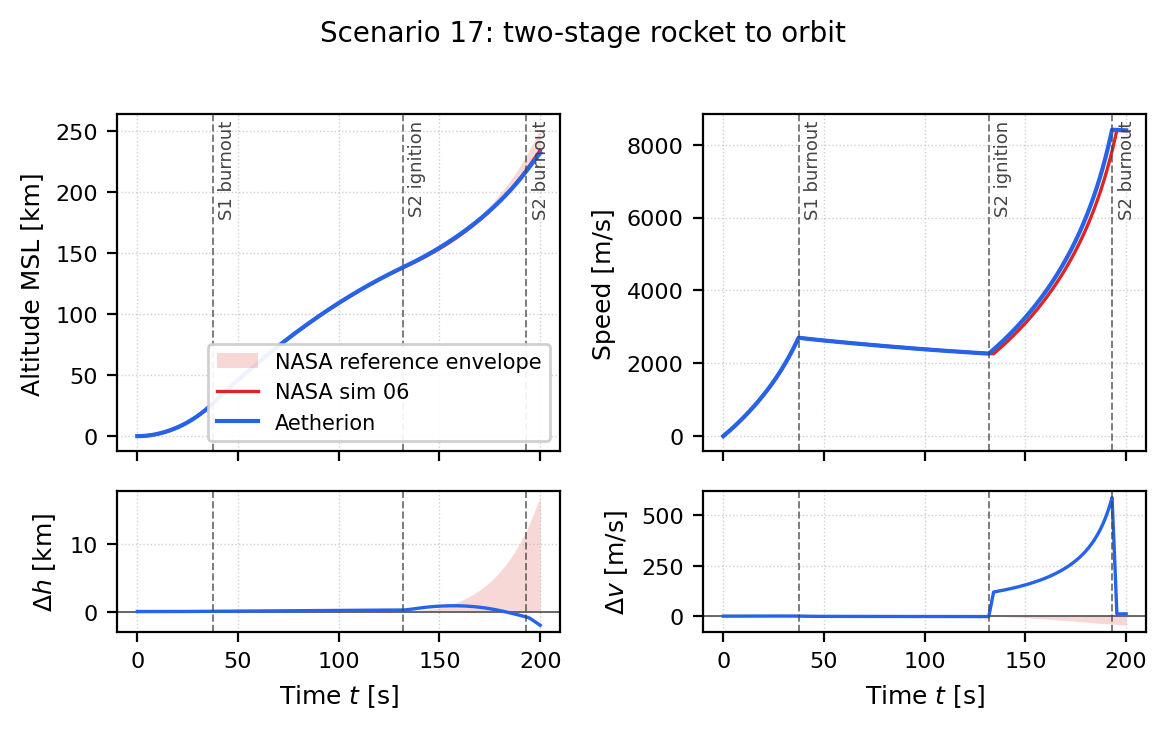
\includegraphics[width=\linewidth]{figures/scenario17}
  \caption{Scenario 17 altitude and speed against the NASA reference runs.  The
    shaded band is the envelope spanned by sims~04, 05 and~06; the lower panels
    give the signed difference of Aetherion from sim~06 on the same band.  The
    altitude difference stays well inside the envelope throughout, and the
    envelope itself widens sharply after S2 ignition.  The speed difference
    opens at S2 ignition, grows through the second burn and collapses at
    burnout, which identifies it as a difference in ignition epoch rather than
    accumulated integration error.  Generated by
    \texttt{papers/eucass/scripts/plot\_scenario17.py}; errors in
    Table~\ref{tab:scenario17_errors} are produced by
    \texttt{scripts/compare\_atmos17\_errors.py} from the same run.}
  \label{fig:scenario17}
\end{figure}

\subsection{Constraint Preservation}
\label{sec:constraint}

A comparison between an implicit RKMK method on $\SE$ and an explicit RK4 on a
flat state varies three things at once---the manifold treatment, the tableau,
and the order---so nothing measured that way can be attributed to the
Munthe-Kaas construction in particular.  We therefore measure the $\SO$
constraint residual $\norm{R^\top R - I}_F$ over a factorial design in which
the tableau and the manifold treatment are varied independently.

All runs use the asymmetric tumbling body of Section~\ref{sec:order_test} over
\SI{600}{\second} at $h = \SI{0.1}{\second}$ (\num{6000} steps).  The flat
baselines carry the same 13-component state
$[q,\,\mathbf{p},\,\omB,\,\vB]$ and, in the implicit cases, solve the same
stage system to the same residual tolerance as the RKMK stepper, using the
identical Butcher tableau; only the coordinate map differs.  Table~\ref{tab:drift}
gives the final residuals and Figure~\ref{fig:constraint_drift} the time
histories.

\begin{figure}[h]
  \centering
  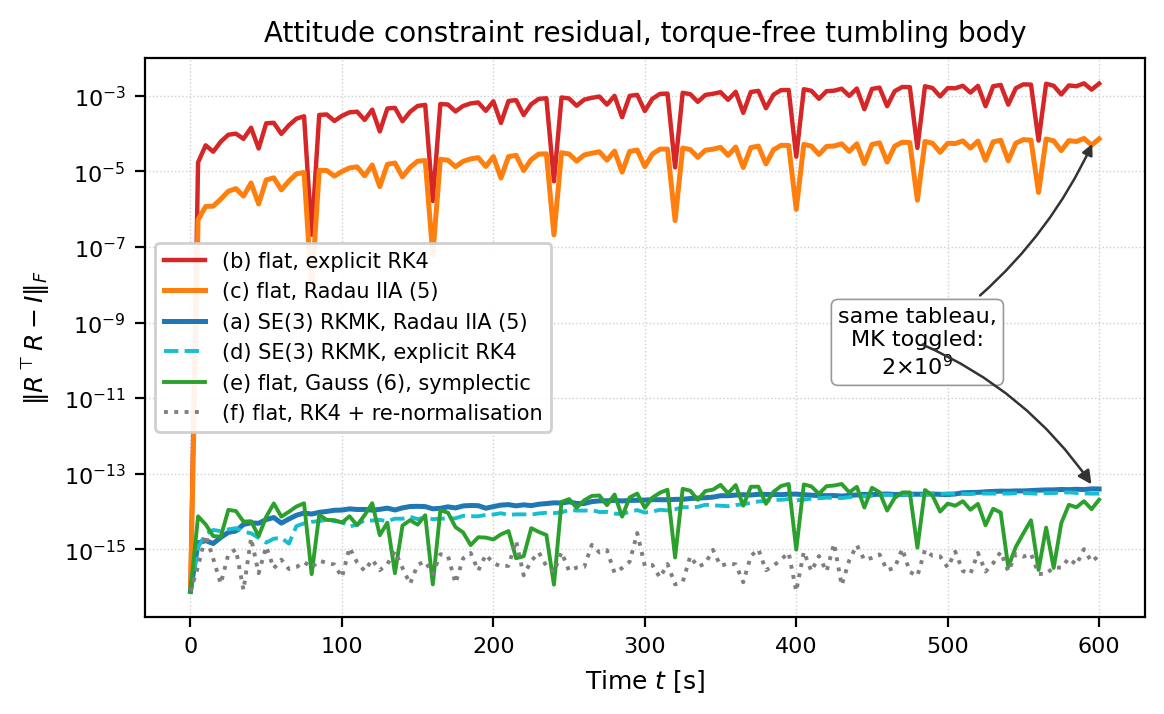
\includegraphics[width=0.78\linewidth]{figures/constraint_drift}
  \caption{Attitude constraint residual over \SI{600}{\second}, for the six
    cells of Table~\ref{tab:drift}.  Both flat-state cells whose tableau is not
    symplectic---RK4~(b) and Radau~IIA~(c)---grow secularly; holding the
    tableau fixed and moving the update onto the group, (c)~$\to$~(a), removes
    the growth entirely.  The two RKMK curves (a,~d) lie together at the
    round-off floor irrespective of tableau, as do the symplectic flat cell~(e)
    and the re-normalised cell~(f).  Generated from
    \texttt{papers/eucass/data/manifold\_factorial\_trace.csv}, emitted by the
    \texttt{[factorial][csv]} regression test.}
  \label{fig:constraint_drift}
\end{figure}

\begin{table}[h]
  \centering
  \caption{Attitude constraint residual $\norm{R^\top R - I}_F$ after
    \SI{600}{\second} ($h = \SI{0.1}{\second}$, \num{6000} steps).  Rows~(a)
    and~(c) differ \emph{only} in the manifold treatment: same tableau, same
    order, same stage-residual tolerance.}
  \label{tab:drift}
  \small
  \begin{tabular}{llllcl}
    \toprule
    & State & Tableau & Order & $\norm{R^\top R - I}_F$ at $T$ & Behaviour \\
    \midrule
    (a) & $\SE$ (RKMK)  & Radau IIA & 5 & $4.0\times10^{-14}$ & bounded round-off \\
    (d) & $\SE$ (RKMK)  & RK4       & 4 & $3.0\times10^{-14}$ & bounded round-off \\
    (c) & flat          & Radau IIA & 5 & $7.2\times10^{-5}$  & secular growth \\
    (e) & flat          & Gauss     & 6 & $2.1\times10^{-14}$ & bounded (symplectic) \\
    (b) & flat          & RK4       & 4 & $2.1\times10^{-3}$  & secular growth \\
    (f) & flat + renorm & RK4       & 4 & $6.9\times10^{-16}$ & bounded (by projection) \\
    \bottomrule
  \end{tabular}
\end{table}

The controlled comparison is (a) against (c).  Holding the Radau~IIA tableau,
the order, and the Newton tolerance fixed and replacing the Lie-group update by
a flat one costs \emph{nine orders of magnitude} in constraint residual.  The
RKMK residual is pure round-off accumulated over the step count---the rotation
factor is a product of exact $\SO$ elements, so there is no truncation
contribution to remove---whereas the flat state leaves the manifold at a rate
set by its truncation error, secularly rather than diffusively.

The remaining rows separate the two factors that the older comparison
conflated.  Going from (b) to (c)---explicit order~4 to implicit order~5, still
flat---improves the residual by a factor of \num{29}, so implicitness and order
account for about \num{1.5} of the nine orders and no more.  Conversely (a)
against (d) shows the same round-off-level residual for an explicit and an
implicit tableau once the update is on the group: with RKMK, manifold
membership does not depend on the tableau at all.

Rows~(e) and~(f) are reported deliberately rather than omitted, because each
reaches the constraint by a route that the orthonormality metric alone cannot
distinguish from~(a).  Per-step re-normalisation~(f) satisfies the constraint,
and to a tighter tolerance than the accumulated matrix product, because $R$ is
rebuilt from a unit quaternion at every step.  Row~(e) is the more interesting
case: $\norm{q}^2$ is a \emph{quadratic} invariant of the quaternion kinematics,
and a Runge-Kutta method conserves every quadratic invariant of its vector
field exactly when
\begin{equation}
  M_{ij} \;=\; b_i a_{ij} + b_j a_{ji} - b_i b_j \;=\; 0
  \qquad \forall\, i,j ,
  \label{eq:cooper}
\end{equation}
a condition satisfied by the Gauss-Legendre family and violated by Radau~IIA.
Measured directly on the two tableaux, $\max_{ij}\lvert M_{ij}\rvert$ is
\num{2.8e-17} for three-stage Gauss and \num{3.7e-2} for three-stage
Radau~IIA, which is precisely why (e) holds the constraint and (c) does not.  A
symplectic tableau therefore attains round-off orthonormality with no
Munthe-Kaas machinery whatever, and any claim that only RKMK can preserve the
manifold would be false.

What distinguishes the RKMK rows is that they achieve this for \emph{any}
tableau, and hence without constraining the choice of tableau on grounds
unrelated to the dynamics.  Section~\ref{sec:stiff_exclusive} shows that this
freedom is not academic: the flat formulation can buy manifold membership only
by adopting a symplectic method, and symplectic methods forfeit exactly the
stiff behaviour that motivated Radau~IIA in the first place.  For (f) the
distinction is different in kind: re-normalisation is a projection applied
outside the integrator, so the trajectory it produces is not the trajectory of
the discrete method whose Jacobian an estimator would linearise, and the
projection's own contribution is absent from that Jacobian.

\subsection{Manifold Membership and Stiff Stability Are Exclusive Without RKMK}
\label{sec:stiff_exclusive}

Row~(e) of Table~\ref{tab:drift} raises an obvious question: if a symplectic
tableau on a flat state already holds the constraint at round-off, what does
RKMK add?  The answer is that condition~\eqref{eq:cooper} is a strong
restriction on the tableau, and it is incompatible with the stiff behaviour for
which Radau~IIA was adopted in the first place (Section~\ref{sec:rkmk}).

Symplectic Runge-Kutta methods are $A$-stable but not $L$-stable.  The stability
function of the three-stage Gauss method is the $(3,3)$ Pad\'e approximant to
$e^z$, for which $\lvert R(z)\rvert \to 1$ as $z \to -\infty$: a stiff transient
is not damped at all in the stiff limit, merely alternated in sign.  Radau~IIA
is $L$-stable, $R(-\infty) = 0$, and stiffly accurate, so it annihilates the
transient in a single step.

To make this concrete we add a linear body-frame damping force
$\mathbf{F}_B = -c\,\vB$ to the same tumbling body, which is the model problem
for stiff aerodynamic damping.  Because the Coriolis term $-\omB \times \vB$ is
norm-preserving, the speed obeys
$\tfrac{\mathrm{d}}{\mathrm{d}t}\norm{\vB}^2 = -2(c/m)\norm{\vB}^2$ exactly, so
\begin{equation}
  \norm{\vB(t)} \;=\; \norm{\vB(0)}\, e^{-(c/m)\,t}
  \label{eq:stiff_exact}
\end{equation}
is available in closed form and no reference integration is required.
Table~\ref{tab:stiff} sweeps the stiffness ratio at fixed
$h = \SI{0.1}{\second}$ and reports the retained fraction
$\norm{\vB(T)}/\norm{\vB(0)}$ after \num{20} steps.

\begin{table}[h]
  \centering
  \caption{Retained fraction $\norm{\vB(T)}/\norm{\vB(0)}$ after \num{20} steps
    at $h = \SI{0.1}{\second}$ ($T = \SI{2}{\second}$) under linear damping, against
    the exact value~\eqref{eq:stiff_exact}.  The last column is the analytic
    amplification factor of the three-stage Gauss tableau, $\lvert R(h\lambda)\rvert$;
    the flat Gauss column reproduces $\lvert R(h\lambda)\rvert^{20}$ to three
    digits, confirming the behaviour is the tableau's and not the solver's.}
  \label{tab:stiff}
  \small
  \begin{tabular}{rrcccc c}
    \toprule
    $c/m$ [\si{\per\second}] & $\lvert h\lambda\rvert$ & exact
      & \shortstack{RKMK\\Radau IIA}
      & \shortstack{flat\\Radau IIA}
      & \shortstack{flat\\Gauss}
      & $\lvert R_{\mathrm{G}}(h\lambda)\rvert$ \\
    \midrule
    $10^{1}$ & $10^{0}$ & $2.1\times10^{-9}$  & $2.1\times10^{-9}$  & $2.1\times10^{-9}$  & $2.1\times10^{-9}$ & 0.368 \\
    $10^{2}$ & $10^{1}$ & $1.4\times10^{-87}$ & $1.3\times10^{-26}$ & $1.9\times10^{-26}$ & $4.4\times10^{-21}$ & 0.096 \\
    $10^{3}$ & $10^{2}$ & $0$                 & $2.6\times10^{-28}$ & $1.2\times10^{-32}$ & $8.2\times10^{-3}$ & 0.787 \\
    $10^{4}$ & $10^{3}$ & $0$                 & $2.4\times10^{-29}$ & $2.5\times10^{-51}$ & $0.619$ & 0.976 \\
    $10^{5}$ & $10^{4}$ & $0$                 & $1.7\times10^{-30}$ & $3.4\times10^{-71}$ & $0.953$ & 0.998 \\
    $10^{6}$ & $10^{5}$ & $0$                 & $2.3\times10^{-31}$ & $3.5\times10^{-91}$ & $0.995$ & 1.000 \\
    \bottomrule
  \end{tabular}
\end{table}

At $\lvert h\lambda\rvert = 1$ the problem is not stiff and all three methods
agree with~\eqref{eq:stiff_exact}.  As the ratio grows the two Radau~IIA columns
drive the transient monotonically further down---this is $L$-stability, and it
is a property of the tableau alone, holding equally with and without the
Munthe-Kaas map.  The Gauss column moves the opposite way, retaining
\SI{62}{\percent}, \SI{95}{\percent} and finally \SI{99.5}{\percent} of the
transient as $\lvert R(h\lambda)\rvert \to 1$.  A single stiffness point would
not reveal this: at $\lvert h\lambda\rvert = 10^2$ the Gauss factor is still
only \num{0.787}, and over a long enough horizon even that decays to
underflow, which would wrongly suggest the method copes.

Combining the two studies on the same stiff problem
($c/m = \SI{1e3}{\per\second}$, $h = \SI{0.1}{\second}$,
$T = \SI{600}{\second}$) gives the summary in Table~\ref{tab:stiff_exclusive}.

\begin{table}[h]
  \centering
  \caption{Manifold membership and stiff transient damping on the same problem.
    Only the RKMK row has both.}
  \label{tab:stiff_exclusive}
  \small
  \begin{tabular}{llcc}
    \toprule
    State & Tableau & $\norm{R^\top R - I}_F$ at $T$ & Stiff transient \\
    \midrule
    $\SE$ (RKMK) & Radau IIA (order 5) & $3.3\times10^{-14}$ & annihilated \\
    $\SE$ (RKMK) & explicit RK4        & \multicolumn{2}{c}{diverges at step 23} \\
    flat         & Radau IIA (order 5) & $7.2\times10^{-5}$  & annihilated \\
    flat         & Gauss (order 6)     & $5.1\times10^{-14}$ & retained \\
    \bottomrule
  \end{tabular}
\end{table}

The flat formulation can have manifold membership or stiff stability but not
both, because the two demand incompatible tableaux: the constraint is held only
by a symplectic method, and the transient only by an $L$-stable one.  Applying
RKMK to the explicit tableau preserves its structure but leaves it with no
stiff stability whatever---it diverges after \num{23} steps.  Only the
Munthe-Kaas update on the $L$-stable, stiffly accurate Radau~IIA tableau
delivers both at once, and Section~\ref{sec:order_test} shows it does so at no
cost in accuracy.  This, rather than orthonormality in isolation, is the
concrete case for the construction.

\subsection{Convergence Order Verification}

Convergence order is established in Section~\ref{sec:order_test}:
Tables~\ref{tab:order_data} and~\ref{tab:order_summary} give the errors and
the fitted slopes, with measured orders of 5.00 (Radau~IIA RKMK) and
3.91--3.98 (explicit RK4 RKMK) against nominal 5 and 4.  The flat-state
Radau~IIA control attains 5.00 as well, and matches the RKMK columns to within
\SI{7}{\percent} at every step size, which is what licenses the reading of
Table~\ref{tab:drift} as a statement about structure rather than about
accuracy.  Figure~\ref{fig:convergence} plots the same data.

\begin{figure}[h]
  \centering
  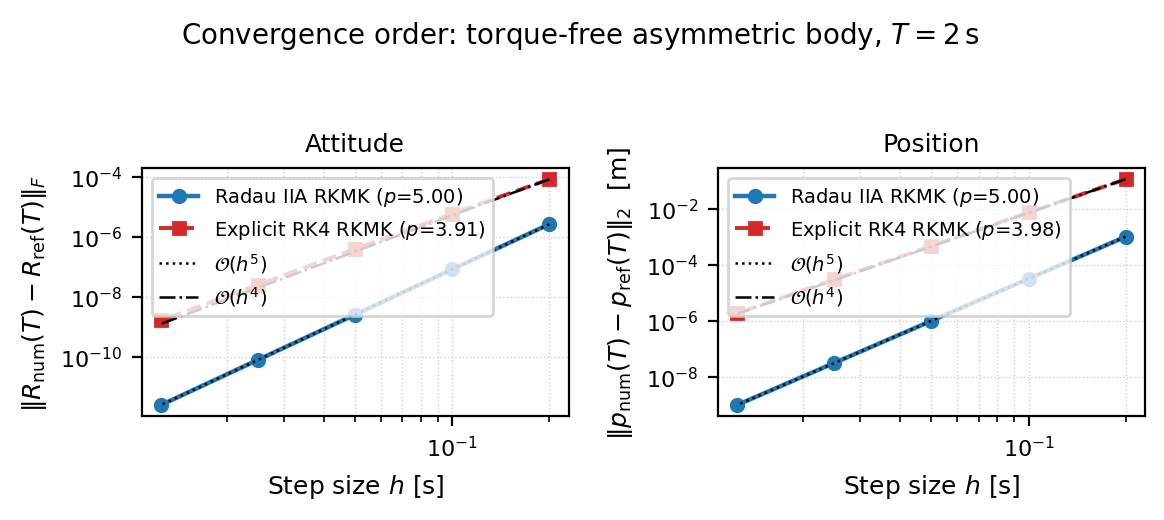
\includegraphics[width=0.72\linewidth]{figures/convergence_order}
  \caption{Global attitude and position error at $T = \SI{2}{\second}$ versus
    step size, torque-free asymmetric body.  Reference slopes $h^5$ and $h^4$
    shown dotted.  Generated from
    \texttt{papers/eucass/data/convergence\_order.csv}, which is emitted by the
    \texttt{[convergence][csv]} regression test.}
  \label{fig:convergence}
\end{figure}

Because both studies are regression tests that emit the data files from which
these figures are produced, a change that degrades the integrator fails the
build rather than silently invalidating a published claim.

% ---------------------------------------------------------------------------
\section{Conclusions}
\label{sec:conclusions}
% ---------------------------------------------------------------------------

This paper has presented an implicit Runge-Kutta-Munthe-Kaas integrator for
6-DOF flight dynamics that operates on the full Special Euclidean group $\SE$.
Its principal result is an attribution rather than a construction:

\begin{quote}
  \emph{The Munthe-Kaas map decouples structure preservation from the choice of
  Butcher tableau.}
\end{quote}

\noindent
That single sentence carries the practical content of the method, and each
half of it is measured.  Holding the tableau, the order, and the Newton
tolerance fixed and varying only the manifold treatment---the controlled
comparison of rows~(a) and~(c) of Table~\ref{tab:drift}---the Munthe-Kaas
update is worth nine orders of magnitude in constraint residual
($4.0\times10^{-14}$ against $7.2\times10^{-5}$ after \SI{600}{\second}) and,
to within \SI{7}{\percent} at every step size tested, nothing at all in
trajectory accuracy.  It is not an accuracy device and does not trade against
accuracy; everything it contributes is structural.

The decoupling is what makes that structural contribution useful, because
preserving the manifold is not by itself exclusive to RKMK.  A symplectic
tableau on a flat state holds $\norm{R^\top R - I}_F$ at round-off as well
(row~(e)), so orthonormality on its own does not identify what a Lie-group
integrator provides.  The difference is in what each approach costs elsewhere.
The flat formulation can buy manifold membership only by adopting a symplectic
method, and symplectic methods are $A$-stable but not $L$-stable: on the stiff
model problem of Section~\ref{sec:stiff_exclusive} the Gauss tableau retains
\SI{99.5}{\percent} of a transient that Radau~IIA annihilates.  A flat
integrator may therefore have manifold membership or stiff stability, but not
both, because the two demand incompatible tableaux.  RKMK grants membership to
whichever tableau the dynamics require---here the $L$-stable, stiffly accurate
Radau~IIA---and so is the only one of the four combinations examined that has
both.

A methodological corollary follows.  A comparison between a Lie-group
integrator and an explicit flat-state one varies the manifold treatment, the
tableau, and the order at the same time, and cannot support a claim about any
one of them however large the gap it reports.  In the present case the
confound proves benign---implicitness and order account for a factor of
\num{29} of the total, and the Munthe-Kaas map for the remaining nine
orders---but that is a measurement, not something the design of such a
comparison could have established.

Supporting these results are four design decisions:

\begin{enumerate}[leftmargin=*, label=(\arabic*)]
  \item \textbf{Single Lie-group treatment}: the pose $g \in \SE$ is updated
    by one $\se$-valued Newton solve and one exponential map, preserving the
    screw-motion coupling between rotation and translation that a split
    $\SO \times \R^3$ approach discards.
  \item \textbf{Fifth-order implicit scheme}: Radau~IIA provides L-stability
    and fifth-order accuracy, enabling step sizes up to \SI{0.1}{s} on stiff
    aerodynamically damped trajectories without accuracy degradation.
  \item \textbf{Exact Jacobians via CppAD}: quadratic Newton convergence is
    achieved on the 18-dimensional stage system without finite-difference
    truncation error.
  \item \textbf{Validated against NASA reference trajectories}: four scenarios
    from TM-2015-218675 confirm correctness of the gravity, aerodynamic, and
    propulsion models across flight regimes from subsonic pull-up to hypersonic
    ballistic re-entry.
\end{enumerate}

Future work will extend the integrator to manifold-consistent discrete extended
Kalman filtering for launch-vehicle state estimation, and to variational optimal
control formulations that exploit the AD-transparent forward pass.  The library
is available as open-source software at the address given in
\citet{aetherion_2025}.

% ---------------------------------------------------------------------------
\section*{Acknowledgements}
% ---------------------------------------------------------------------------

The author thanks the NASA Engineering and Safety Center (NESC) for making the
reference simulation data from TM-2015-218675 publicly available.

% ---------------------------------------------------------------------------
% Bibliography
% ---------------------------------------------------------------------------
\bibliographystyle{unsrtnat}
\bibliography{references}

% ---------------------------------------------------------------------------
% Appendix
% ---------------------------------------------------------------------------
\appendix

\section{Coefficients of the $Q$ Term in $\dexp^{-1}_\xi$}
\label{app:dexp_coeffs}

The scalar coefficients in equation~\eqref{eq:Q_term} are, for
$\theta = \norm{\omega}$:
\begin{align}
  c_1 &= \frac{\theta - \sin\theta}{\theta^3}, \\
  c_2 &= \frac{\theta^2 + 2\cos\theta - 2}{2\theta^4}, \\
  c_3 &= \frac{2\theta - 3\sin\theta + \theta\cos\theta}{2\theta^5}.
\end{align}
For $\theta \to 0$ the Taylor expansions are
\begin{align}
  c_1 &\approx \tfrac{1}{6} - \tfrac{\theta^2}{120} + O(\theta^4), \\
  c_2 &\approx \tfrac{1}{12} - \tfrac{\theta^2}{180} + O(\theta^4), \\
  c_3 &\approx \tfrac{1}{120} - \tfrac{\theta^2}{1260} + O(\theta^4).
\end{align}
These series are used in the implementation whenever $\theta^2 < 10^{-6}$ to
avoid catastrophic cancellation.

\section{Radau IIA Stage Residual: Full Scalar Form}
\label{app:residual_scalar}

For completeness, the full scalar form of residual~\eqref{eq:residual} for
$s = 3$ stages is:

For $i = 1,2,3$:
\begin{equation}
  r_i = \xi_i - h\;\dexp^{-1}_{\eta_i}(t_0 + c_i h,\; g_0 \cdot \Exp(\eta_i),\; x_0 + \rho_i),
\end{equation}
where $\eta_i = \sum_j a_{ij}\xi_j$, $\rho_i = \sum_j a_{ij} k_j$, and
$\dexp^{-1}$ is the $6\times6$ matrix~\eqref{eq:dexp_inv}.  The stacked
system $[r_1^\top, r_2^\top, r_3^\top]^\top = \mathbf{0}$ has $18$ scalar
equations in $18$ unknowns $[\xi_1^\top, \xi_2^\top, \xi_3^\top]^\top$.

\end{document}
